\documentclass[times, twocolumn]{article}
\usepackage{graphicx} % Required for inserting images
\usepackage{subcaption}
\usepackage{amsmath}
\usepackage{float}
\usepackage{pgfplots}
\usepackage{subcaption}
\usepackage{comment}
\usepackage[a4paper, total={7in, 9in}]{geometry}
\usepackage{biblatex}

\addbibresource{mybib.bib}

\title{Spotify Tracks Genre Classification}
\author{Nabeha Barkatullah, Mia Striebeck, Laksha Karthikeyan, Carson Chiem, Shuzo Naruse}
\date{May 20, 2024}

\begin{document}
\maketitle

\newpage
% abstract
\begin{abstract}
Discovering new music that fits within your music taste is time-consuming and difficult. On top of there being an abundance of music to sift through, finding songs from the bulk that you actually enjoy listening to can go either way. With this project, we aim to utilize a Spotify dataset to build a model to classify songs under genres, with the potential of being part of a song recommendation system. Using the attributes from the dataset, such as the relevant music listening patterns and classification of songs, we will predict the genre a song falls under. Our goal is to build a classification model that predicts a song’s genre based on user-inputted track features.
\end{abstract}
\section{Introduction}
[include intro]
% background
\section{Background}
%literature review
\section{Literature Review}

\section{Dataset Description and Modeling Approach}
The selected Kaggle dataset contains data on Spotify songs from over 125 genres, with each song having associated characteristics. This set contains around 114k data points condensed in a CSV format, with 20 features. These features are related to track identification, classification, and characteristics of the track (ie: tempo and time signature). In full, the features are track id, artists, album name, track name, popularity, duration (ms), explicit, danceability, energy, key, loudness, mode, speechiness, acousticness, instrumentalness, liveness, valence, tempo, time signature, and track genre.

\section{Exploratory Data Analysis}
The main purpose of Exploratory Data Analysis (EDA) is to help look at data before making any assumptions. It can help identify obvious errors, better understand patterns within the data, detect outliers, or find interesting relations among the variables.

\subsection{Visualizing the Dataset}
Creating distributions of the data can help visualize whether the data is skewed such as towards a gender or age group, as skewness can lead to biased parameter estimates or inaccurate predictions.

% adding Figure 1 - image of feature distributions
\begin{figure}[H]
    \centering
    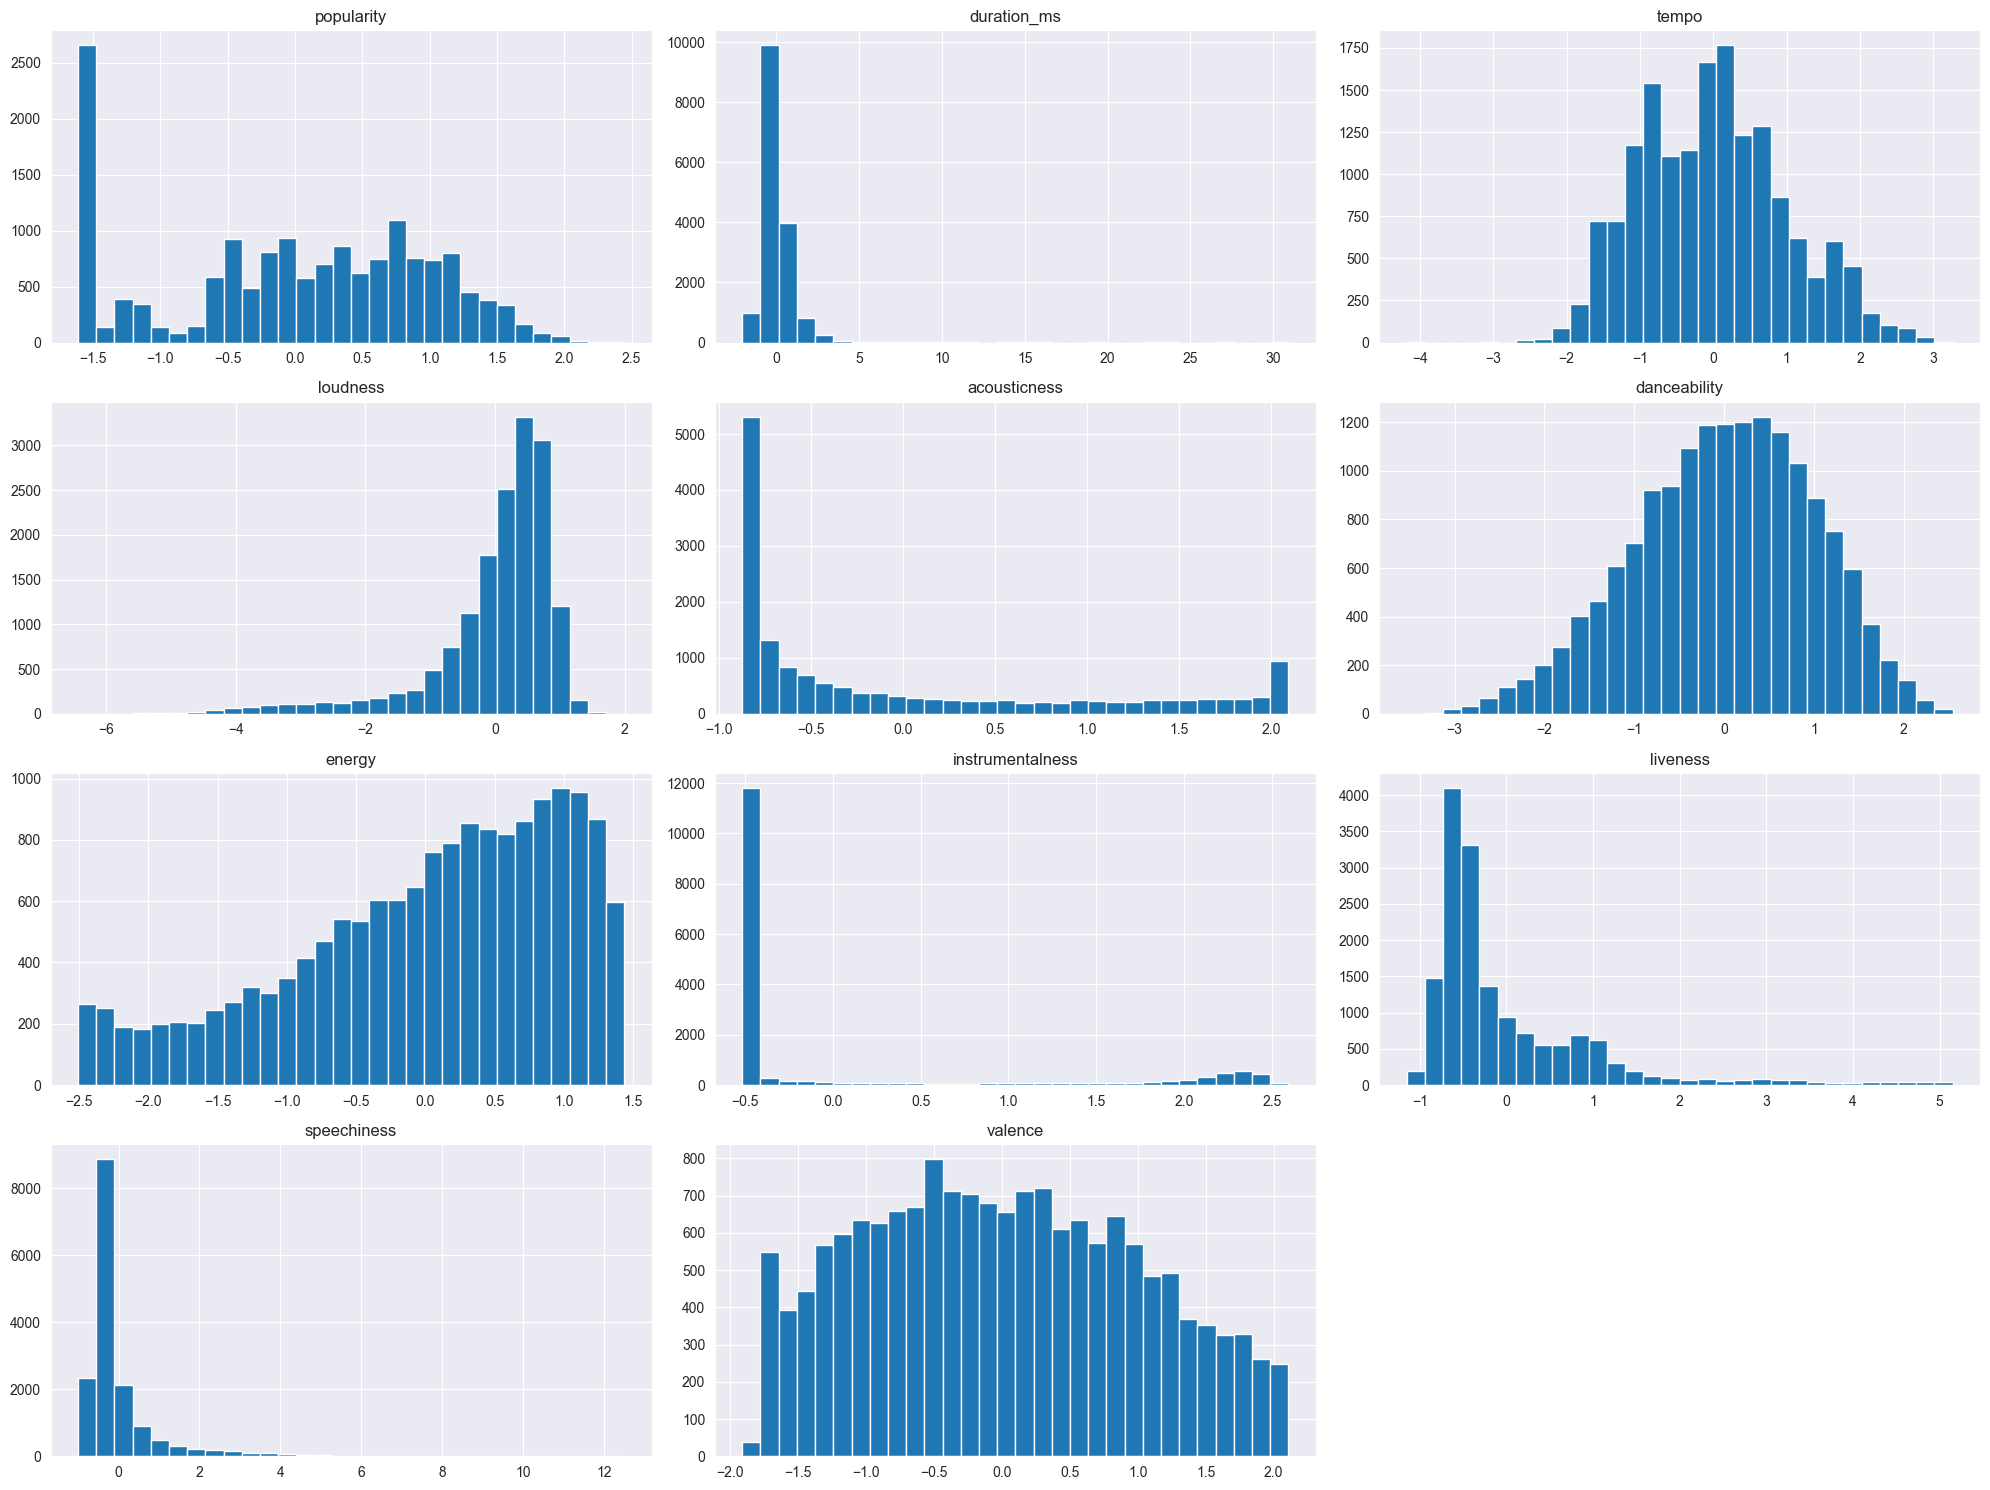
\includegraphics[width=0.55\textwidth]{feature_dists.png}
    \caption{Caption}
    \label{graph:dists}
\end{figure}

As shown in Figure \ref{graph:dists}, the danceability and tempo have nearly normal distributions. The loudness, acousticness, speechiness, liveliness are skewed, with loudness being left-skewed and the rest being right-skewed. For popularity, if the songs with the value 0 are taken out, the distribution would almost be normal. Also, energy has an increasing distribution.

% adding Figure 2 - boxplots
\begin{figure}[H]
    \centering
    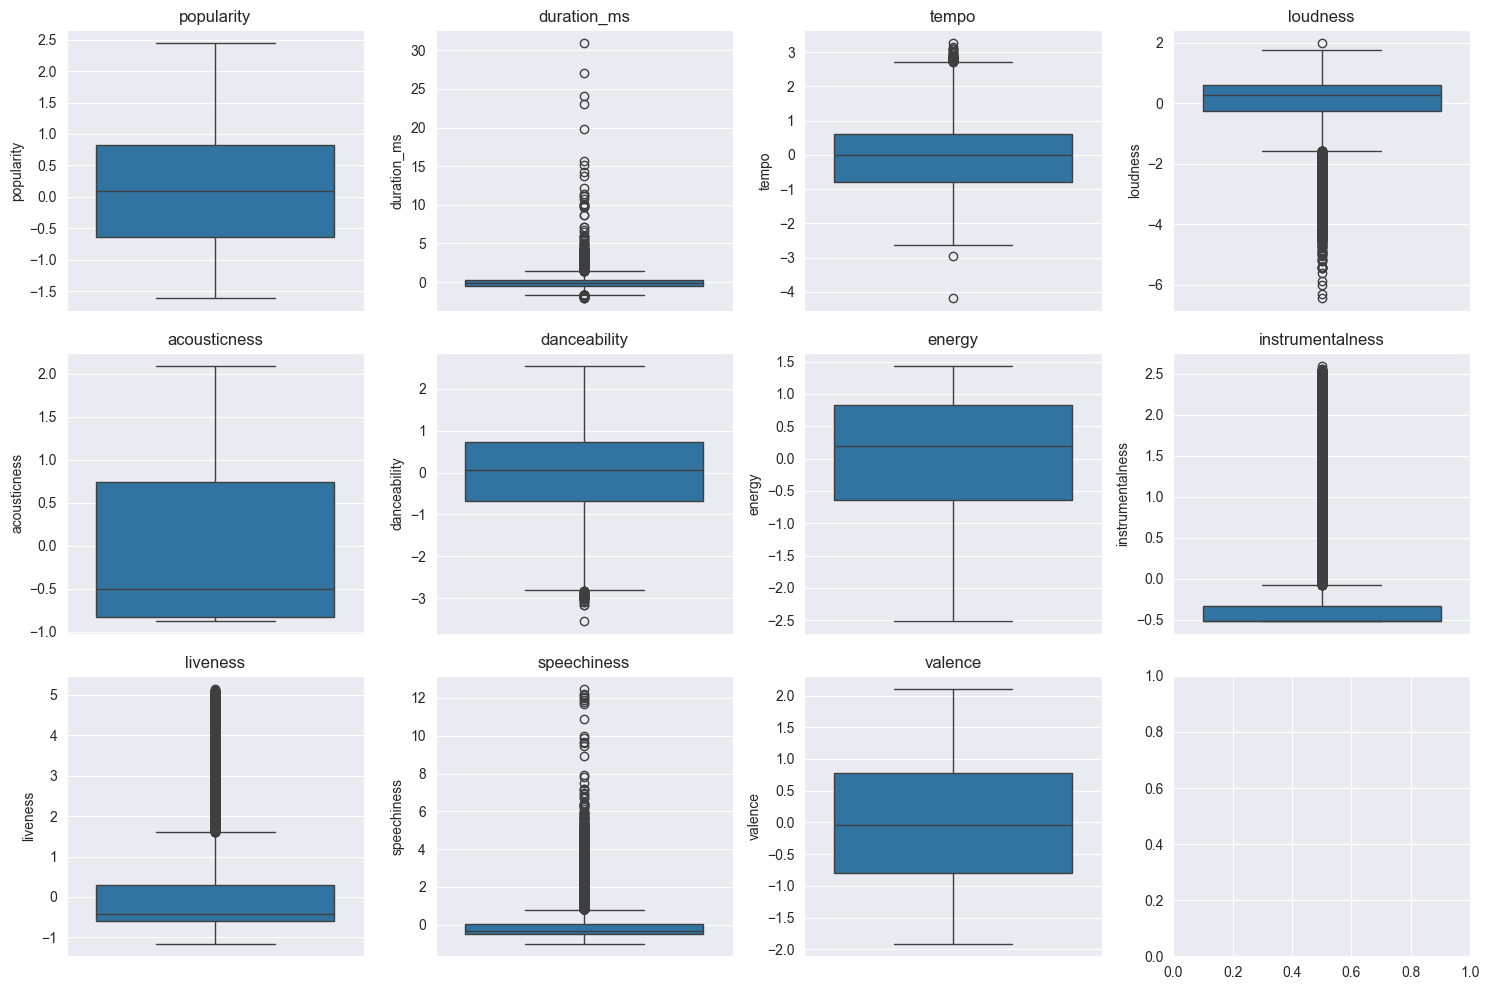
\includegraphics[width=0.5\textwidth]{feat_boxplots.png}
    \caption{Caption}
    \label{Boxplots}
\end{figure}

Box Plots can also be used to visualize skewed data and identify outliers.
The box plots in Figure \ref{Boxplots} map the distributions for ...\\
- acousticness, energy and valence have no outliers\\
- all of the other features have many outliers which makes sense since they are features that describe a song and are thus useful and should be kept to keep the diversity of the songs in the dataset\\
It's also good to note the absence of outliers, as the presence of outliers may cause problems during model fitting. Since our data is clean, we can better avoid inflated error metrics that can significantly impact model performance by skewing parameter estimates.

\subsection{Feature Selection} Feature selection is the process of choosing the most relevant features to use in our machine learning algorithm. The main goal of feature selection is to improve the performance of a predictive model while also reducing the computational cost of modeling.\\

One way to go about choosing relevant features is by using the Filter Method~\cite{HeavyAI}. The Filter Method can be used to filter out the features and take only a relevant subset of features~\cite{HeavyAI}. We employed Pearson's Correlation Coefficient (\ref{eq:pearson}) and Spearman's Correlation Coefficient (\ref{eq:spearman}) to determine the correlations between features and lung cancer severity.\\


In examining the correlation coefficients between the various features and lung cancer severity levels in Figure \ref{table:rel_feats}, we aim to identify the \\

In addition to understanding the correlations between the features and music genre or idk, it's important to understand the correlations \textit{between} the features in building accurate models. Correlations between features provide insights into how the variables in the dataset interact with each other, which can guide feature selection, model construction, and interpretation of results. While strong correlations between features may indicate redundancy or multicollinearity*, leading to potential model instability or overfitting, they can also highlight important relationships that contribute to the predictive power of the model. Therefore, it is essential to examine the feature correlations for making informed decisions about whether to keep or remove features based on the specific context of the ML problem and the goals of the analysis.\\

\begin{figure}[H]
    \centering
    \textbf{Pearson's Correlation Heatmap of Relevant Features}
    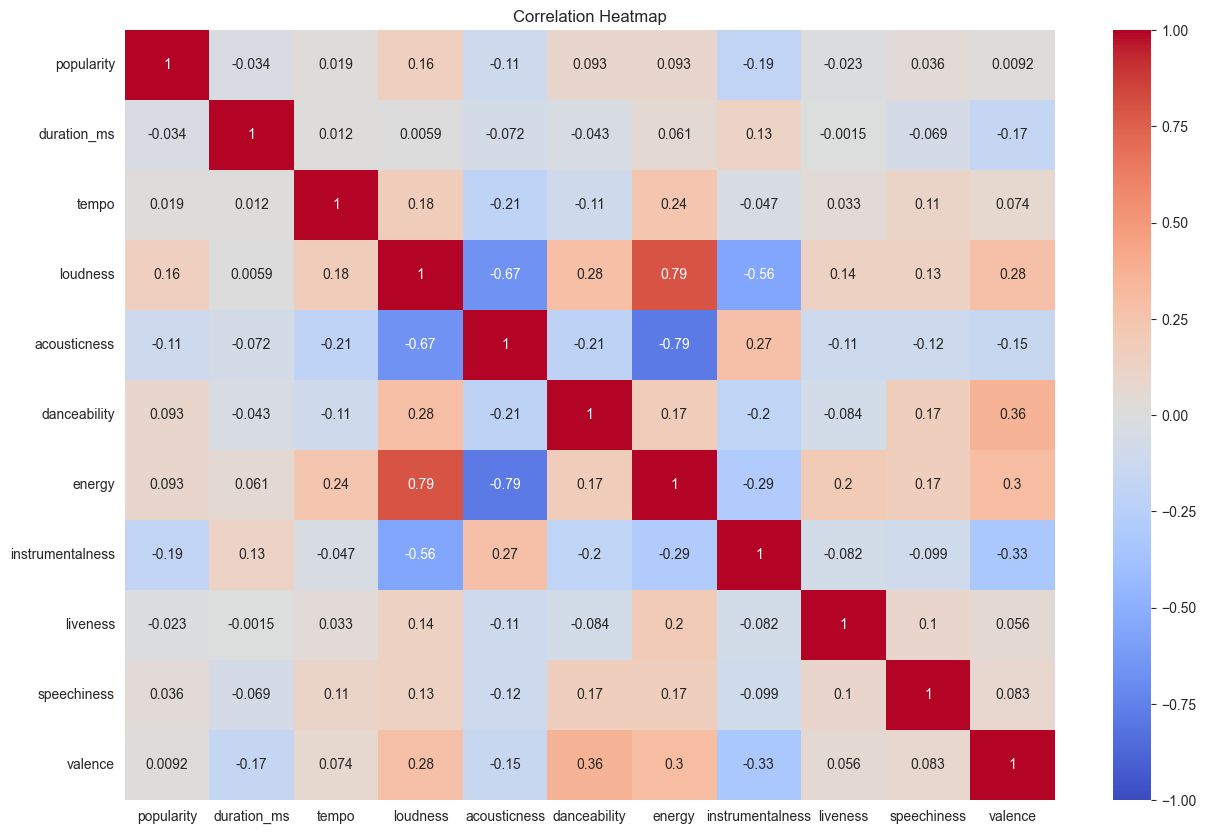
\includegraphics[width=1.0\linewidth]{corr_heatmap.png}
    \caption{The Pearson's correlation heatmap depicts the pairwise correlations between the 13 relevant features identified through the Filter Method. Each cell in the heatmap represents the correlation coefficient between two features, ranging from -1 to 1. A value close to 1 indicates a strong positive correlation, while a value close to -1 suggests a strong negative correlation. A correlation of 0 indicates no linear relationship between the features. This heatmap provides insights into the interplay between different features, guiding feature selection and model interpretation.}
    \label{heatmap}
\end{figure}

Despite observing both weak and strong correlations among the 13 features in Figure \ref{heatmap}, words.

\section{Model Construction}
Based on our exploratory data analysis, we determined that the relevant features that are potentially useful in predicting lung cancer severity are air pollution, alcohol use, dust allergy, occupational hazards, genetic risk, chronic lung disease, balanced diet, obesity, smoking, passive smoker, chest pain, coughing of blood, and fatigue. These factors will become the inputs (X) of our predictive model.

\section{Results}
\subsection{Model Performances}


\subsection{Model Implications}

\section{Discussion}

\section{Conclusion}

\printbibliography


\end{document}
